% Correlation Plot: Output Length vs ROUGE-1
\begin{figure}[t]
\centering
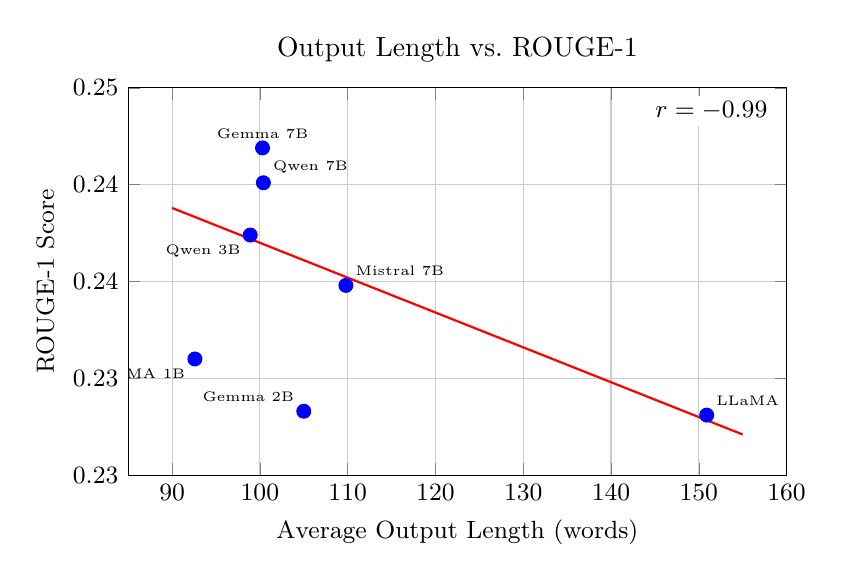
\begin{tikzpicture}
\begin{axis}[
    width=0.82\textwidth,
    height=6.5cm,
    xlabel={Average Output Length (words)},
    ylabel={ROUGE-1 Score},
    xmin=85, xmax=160,
    ymin=0.225, ymax=0.245,
    grid=both,
    grid style={gray!20},
    major grid style={gray!40},
    tick label style={font=\small},
    label style={font=\small},
    title={Output Length vs.\ ROUGE-1},
    title style={font=\normalsize},
]

% Data points
\addplot[
    only marks,
    mark=*,
    mark size=2.5pt,
    blue
] coordinates {
    (150.9,0.2281)
    (100.4,0.2401)
    (109.8,0.2348)
    (98.9,0.2374)
    (92.6,0.2310)
    (105.0,0.2283)
    (100.3,0.2419)
};

% Regression line (fitted visually from data)
\addplot[
    red,
    thick,
    domain=90:155,
    samples=100
]
{0.255 - 0.00018*x};

% Labels
\node[font=\tiny, anchor=south west]
at (axis cs:150.9,0.2281) {LLaMA 3B};

\node[font=\tiny, anchor=south west]
at (axis cs:100.4,0.2401) {Qwen 7B};

\node[font=\tiny, anchor=south west]
at (axis cs:109.8,0.2348) {Mistral 7B};

\node[font=\tiny, anchor=north east]
at (axis cs:98.9,0.2374) {Qwen 3B};

\node[font=\tiny, anchor=north east]
at (axis cs:92.6,0.2310) {LLaMA 1B};

\node[font=\tiny, anchor=south east]
at (axis cs:105.0,0.2283) {Gemma 2B};

\node[font=\tiny, anchor=south]
at (axis cs:100.3,0.2419) {Gemma 7B};

% Correlation coefficient
\node[
    anchor=north east,
    fill=white,
    inner sep=2pt,
    font=\small
]
at (rel axis cs:0.98,0.98)
{$r=-0.99$};

\end{axis}
\end{tikzpicture}

\caption{
Relationship between average output length and ROUGE-1 score across the multi-agent architecture for all seven models. A strong negative correlation ($r=-0.99$) is observed, indicating that shorter summaries tend to achieve higher lexical overlap with reference summaries. This analysis is limited to multi-agent outputs; the same relationship may or may not hold for baseline outputs.
}
\label{fig:length_rouge_correlation}
\end{figure}